\documentclass[11pt]{article}

\usepackage{../styles/arxiv}

\usepackage{../styles/pgfgantt}
\usepackage{../styles/bibtopic}

\usepackage[latin1]{inputenc}
\usepackage{tikz}
\usetikzlibrary{shapes,arrows, fit}

\tikzstyle{block} = [rectangle, draw, fill=black!10,
  text width=5em, text centered, rounded corners, minimum height=4em]
\tikzstyle{line} = [draw, -latex']
\tikzstyle{file} = [rectangle, draw, fill=black!20, minimum height=2em,
  text width=5em, text centered]
\tikzstyle{bin} = [circle, draw, fill=black!30, minimum height=3em,
  text width=5em, text centered, inner sep=0pt]

\usepackage{setspace}

\renewcommand{\baselinestretch}{1.333}

\newcommand{\undertitle}{Progress Report}

\title{Extending Just-in-Time Compilation for OP2}

\author{Nathan Dunne - u1604486}

\begin{document}
\maketitle

\section*{Introduction}
The aim of this project is to contribute to the OP2 open-source project\cite{OP2rep}, an Embedded Domain Specific Langauge for developing unstructured mesh based applications. It provides a programmer access to greater performace using an abstraction from hardware specific optimisations, OP2 also provides the further benefit of allowing portability between different platforms, allowing all programs written using the API to utilise the latest hardware generation by simply updating the OP2 code generation. 
\par On top of the existing work, there is space for greater performance to be gained through the use of Just-In-Time (JIT) compilation: re-compiling the source code at run-time once the inputs are known, to allow expensive repeated operations to be replaced with static constants where possible, expanding the ability of the compiler to optimise through constant propogation and other methods. This can provide significant benefit, especially over a large number of iterations as a small improvement per-iteration can compound to better offset the one-time cost of the re-compilation. 
\par The inputs to the program will be the description of the unstructured mesh as an input file, which is read at runtime. Since this information is not known to the compiler ahead of time, it is only possible to optimise based on this information "Just In Time", or immediately before execution.
\par The sequential JIT code generator has already been completed, so the primary goal is to target the NVIDIA GPU architecture using CUDA, attempting to reach a performance improvement over Ahead-of-Time compiled CUDA generation. Since the OP2 API itself will not be modified by the project, existing applications can be used to benchmark performance. Primarily this will be Airfoil \cite{airfoil}, an industrially representative computational fluid dynamics (CFD) program, and later VOLNA\cite{volna}, a non-linear shallow water equation solver. Both use the C OP2 API.
\subsection*{Motivations}
The motivations behind this project are a desire to use and expand on knowledge of optimisations and high-performance computing gained in the second year \textit{Advanced Computer Architecture} module, as well as an interest in compilers and code generation. It will also be personally beneficial to gain experience contributing to a real open-source project, with an existing code base to deal with. It is gratifying to know that if the project is completed to a high standard, it could be merged into the master branch and used beyond the submission for a module.
\par The decision to target GPUs is as a result of the increased need for parallelism in high performance computing systems and applications. GPUs are in nature aimed at graphics processing, which requires many operations to be performed in parallel, but similarly many HPC programs (including unstructed mesh apps like CFD programs) can benefit from this architecture now that they are capable of double precision.
\clearpage
\section*{Research}
In order to begin contributing to the OP2 source, I needed to build an understanding of the existing work. There are 2 main sources for this information:
\begin{itemize}
 \item{Papers publish on the OP2 website}
 \item{Analysis and Benchmarking of existing source code}
\end{itemize}
While academic papers are useful to understand the context of the project and the motivations behind it \cite{op2main} \cite{autoVector} \cite{industrial}; the existing code gives a more concrete understanding of the implementation, and the form my contributions will take. Understanding the basic structure of an OP2 program, where data is divided into sets and mappings between them - and loops can be defined as a seperate "kernel" of operations, is critical to making a useful contribution. 


\section*{Technical Content}
\subsection*{Existing Work}
It should be noted, the term "Just-In-Time Compilation" in the case of this project doesn't strictly mean the same thing it's usual definition, for example in the JVM where the intermediate representation bytecode is compiled to native machine code at run time, allowing optimisation of bytecode to take the inputs into account. In this project, the Ahead-Of-Time compiled executable issues a make command during the run of the program, so that loop functions can be generated with constants defined in the input file as a macro that can be expanded by the preprocessor. This can only be done at runtime, and should provide perfomance benefit over retrieving a value from memory.

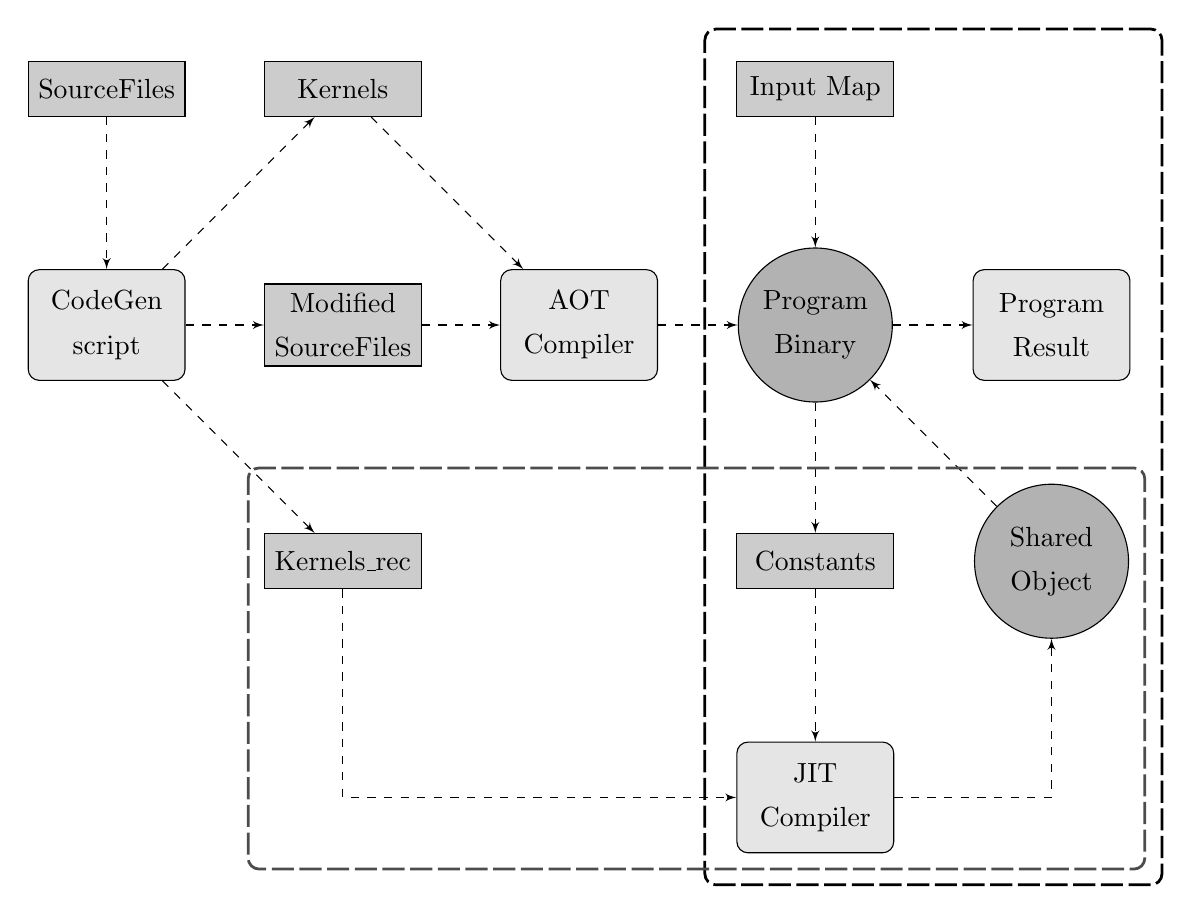
\begin{tikzpicture}[node distance=3cm, auto]

  \node [file] (source) {SourceFiles};
  \node [block, below of=source] (op2py) {CodeGen script};
  \node [file, right of=op2py] (sourceOp) {Modified SourceFiles};
  \node [file, above of=sourceOp] (Kernels) {Kernels};
  \node [file, below of=sourceOp] (recKernels) {Kernels\_rec};
  \node [block, right of=sourceOp] (aot) {AOT Compiler};

  \node [bin, right of=aot] (binary) {Program Binary};
  \node [file, above of=binary] (input) {Input Map};
  \node [file, below of=binary] (consts) {Constants};
  \node [block, below of=consts] (jit) {JIT Compiler};
  \node [bin, right of= consts] (so) {Shared Object};
  \node [block, right of=binary] (result) {Program Result};

  \path [line, dashed] (source) -- (op2py);
  \path [line, dashed] (op2py) -- (recKernels);
  \path [line, dashed] (op2py) -- (sourceOp);
  \path [line, dashed] (op2py) -- (Kernels);
  \path [line, dashed] (sourceOp) -- (aot);
  \path [line, dashed] (Kernels) -- (aot);
  \path [line, dashed] (aot) -- (binary);
  \path [line, dashed] (input) -- (binary);
  \path [line, dashed] (binary) -- (consts);
  \path [line, dashed] (recKernels) |- (jit);
  \path [line, dashed] (consts) -- (jit);
  \path [line, dashed] (jit) -| (so);
  \path [line, dashed] (so) -- (binary);
  \path [line, dashed] (binary) -- (result);

  \tikzset{dotted box1/.style={draw=black!100, line width=1pt, dash pattern=on 8pt off 2pt,
    inner sep=4mm, rectangle, rounded corners}};

  \tikzset{dotted box2/.style={draw=black!70, line width=1pt, dash pattern=on 8pt off 2pt,
    inner sep=2mm, rectangle, rounded corners}};

  \node (runtime) [dotted box1, fit = (input) (jit) (result)] {};
  \node (runtime) [dotted box2, fit = (recKernels) (so) (jit)] {};

\end{tikzpicture}

As well as the research above, the following work has been completed so far.
\subsection*{Prerequisites and Tools}
OP2 utilises two well established parallel mesh partitioning libraries: ParMetis\cite{metis} and PT-Scotch\cite{scotch}. As I intend to work mainly on my personal laptop, a version of each had to be retrieved and built with the correct build arguments. The work with CUDA also required the CUDA Software Development Kit\cite{cuda}, and drivers for the Nvidia MX250 card I have available. Finally, the airfoil example application makes use of HDF5 file I/O operations, so a build of that library was required as well. 
\par
The project is hosted on GitHub, with a branch created to manage my contributions. This will allow me some saftey in the case of  
\subsection*{CUDA familiarity}
Since the CUDA c++ API is not something I have used before, I experimented with writing small programs to run on a gpu, as well as referencing the \textit{Nvidia CUDA C Programming Guide} to build my Understanding. Knowledge of how CUDA programs can solve common problems in parallelism, such as local and global shared memory, and the use of \textit{syncthreads()} will undoubtably be necessary to complete this project.

\subsection*{Hardware Resource}
The graphics card in my personal laptop is sufficent to execute the generated CUDA code, and ensure correctness, however the system will be too noisy to gather representative benchmarks. To this end, I applied for and have been granted access to the Orac Hight Performance Computing node in the department, which will be used only for benchmarking.

\subsection*{Existing code familiarity}
The existing JIT work was done in the branch \textit{lazy-execution} of the Git repository. In order to extend this work, I've rebased the branch onto the master branch in order to benefit from the many changes commited to master since they diverged. 
\par Once this was done, I could begin to understand what the existing code does and how my code fits in. I was already aware that the bulk of my work will be done in the "translator" folder, with C as the target and python as the script language. Starting here with the main \textit{op2.py} script makes sense. This script parses the input file for API calls such as \textit{op\_decl\_set()}, \textit{op\_decl\_const}, and \textit{op\_par\_loop()}; for declaring sets, constants and loops respectively. These are sections that will need to be replaced for a normal compiler to accept them.
\par Each one is checked to be well formed, and the information described in their parameters recorded. This is especially important for loops, where the number of arguments and the type of each argument is defined, as well as whether it is optional, and stored in the list of "kernels". In order to be valid, each kernel must also have a definition of the operations to perform on each iteration, which for the example application \textit{airfoil} is a seperate header file of the same name, but this is not required.
\par The original input file is then written out, with declarations for functions representin each loop with the right number of parameters, and in the place of the loops: calls to these function. The definitions will be generated by the code generation scripts. 
\par op2.py then calls each codegen script for all the supported backends, to generate a folder for each backend containing the generated code. For JIT, initially only op2\_gen\_seq\_jit existed, so my contribution will be to populate this list of code generators similar to the Ahead-of-Time list. The reason for all this analysis of the op2.py script, is to understand the state of the file when the code I write is called, and the parameters that it will recieve:
\begin{enumerate}
\item{masterFile: the name of the first file passed to op2.py}
\item{date: the date today}
\item{consts: master list of declared constants in source file}
\item{kernels: master list of loop kernels declared in source file}
\end{enumerate}
The code generator can then loop through the kernels, and generate a function to call for each one based on the target hardware.

\subsection*{Implementation}
At time of writing the implementation of CUDA JIT code generation has just started. The op2.py script has been modified to call a CUDA\_jit code generation file, and added to the makefile of airfoil to include an airfoil\_CUDA\_jit entry, however the codegeneration itself is still sequential. To complete the CUDA JIT implentation I will use the AoT CUDA implementation as a guide to speed up the process. The work is available in my \textit{feature/jit} branch of the remote repository.

\section*{Reflection and Project Management}
The timetable from the project specification (Figure \ref{fig:orig}) shows the expected level of progress at this stage. In retrospect, It is clear that the original timetable was ambitious, as the project has not run quite to time. While I am still confident that the CUDA JIT code generation can be done by the end of the end of the autumn term (as originally agreed with my supervisor), I have reworked the timetable with a greater allocation of time given to research, and three iterations of longer implementation blocks with one week testing, rather than five rounds of 3 week blocks. Now having a greater understanding of the project, I think it unreasonable to suggest there would a feature worth spending a week testing and benchmarking completed every 2 weeks of development. See Figure \ref{fig:new}. As well as aligning with the end of the Autumn term, this also allows for two more weeks development of time overall.
\par I would attribute the need for an extension to research time to taking an ad hoc approach to working on the project, which has resulted in not putting as much time in as I had planned, instead focussing on closer deadlines. As such I have decided that for next term I will set a weekly timetable of allocated time to work on the project.
\par The timetable aside, other elements of the project haven't provided any significant unexpected issues. All tools and libraries are functioning and compatible.

\section*{Ethics and Risks}
As mentioned in the Project Specification, there are no obvious social or ethical issues with the project, as it will not require the collection or storage of any personal data. It is important to consider the lisence under which the open source project is held, which permits redistribution of the source and binary, as long as it contains the copyright disclaimer.
\par I am also now aware of the Acceptable Use Policy\cite{aup} for the computing facilities provided bt the SCRTP, so I will also ensure to abide by this when benchmarking using Orac.

\newcommand\w{25}
\begin{figure}[p]
\centering
\makebox[0pt]{
\begin{ganttchart}[
expand chart=1.22\textwidth,
vgrid={*3{white},*1{dotted}, *{14}{white}, *1{dotted}, *1{white}, *1{dotted}, *5{white}},
hgrid=true,
y unit chart=0.8cm,
inline,
today=6,
today label=Expected Progress,
today label font=\itshape,
]{0}{\w}

 \gantttitle{Timeline}{26} \\
 \gantttitlelist{0,...,\w}{1} \\

 \ganttgroup{Research}{1}{3} \\ %0%
 
 \ganttset{inline=false}
 \ganttbar{Read Papers}{1}{2}          %1%
 \ganttset{inline=true}

 \ganttgroup{Implementation}{4}{18} \\ %2%

 \ganttset{inline=false}
 \ganttbar{Familiarity Work}{2}{3}     %3%
 \ganttset{inline=true}

 \ganttgroup{Benchmarking}{19}{20} \\  %4%

 \ganttset{inline=false} 
 \ganttbar{Feature Development}{4}{5}  %5%
 \ganttbar{} {7}{8}                   %6%
 \ganttbar{} {10}{11}                  %7%
 \ganttbar{} {13}{14}                  %8%
 \ganttbar{} {16}{17}                  %9%
 \ganttset{inline=true}
 \ganttgroup{Documentation}{21}{25} \\ %10%

 \ganttset{inline=false} 

 \ganttbar{Feature Testing}{6}{6}      %11%
 \ganttbar{}{9}{9}                   %12%
 \ganttbar{}{12}{12}                   %13%
 \ganttbar{}{15}{15}                   %14%
 \ganttbar{}{18}{18}                   %15%

\\
 
 \ganttbar{Results Gathering}{19}{19}  %16%
 \\
 \ganttbar{Results Processing}{19}{20} %17%
 \\  
 
 \ganttbar{Final Report}{21}{25} \\    %18
 \ganttbar{Presentation}{21}{22}       %19

 \ganttlink{elem3}{elem5}
 \ganttlink{elem5}{elem11}
 \ganttlink{elem11}{elem6}
 \ganttlink{elem6}{elem12}
 \ganttlink{elem12}{elem7}
 \ganttlink{elem7}{elem13}
 \ganttlink{elem13}{elem8}
 \ganttlink{elem8}{elem14}
 \ganttlink{elem14}{elem9}
 \ganttlink{elem9}{elem15}
 \ganttlink{elem15}{elem16}
 \ganttset{link mid=0.25}
 \ganttlink{elem15}{elem17}
 \ganttset{link mid=0.5}
 \ganttlink{elem17}{elem18}
 \ganttset{link mid=0.25}
 \ganttlink{elem17}{elem19}
 \ganttset{link mid=0.5}
 \ganttlink{elem1}{elem3}
\end{ganttchart}
}
\caption{Original Timetable}
\label{fig:orig}
\end{figure}
\begin{figure}[p]
\centering
\makebox[0pt]{
\begin{ganttchart}[
expand chart=1.22\textwidth,
vgrid={*{1}dotted, *4{white},*1{dotted}, *{12}{white}, *1{dotted}, *1{white}, *1{dotted}, *5{white}},
hgrid=true,
y unit chart=0.8cm,
inline,
today=6,
today label=Actual Progress,
today label font=\itshape,
]{0}{\w}

 \gantttitle{Timeline}{26} \\
 \gantttitlelist{0,...,\w}{1} \\

 \ganttgroup{Research}{1}{5} \\ %0%
 
 \ganttset{inline=false}
 \ganttbar{Read Papers}{1}{2}          %1%
 \ganttset{inline=true}

 \ganttgroup{Implementation}{6}{18} \\ %2%

 \ganttset{inline=false}
 \ganttbar{Familiarity Work}{2}{5}     %3%
 \ganttset{inline=true}

 \ganttgroup{Benchmarking}{19}{20} \\  %4%

 \ganttset{inline=false} 
 \ganttbar{Feature Development}{6}{8}  %5%
 \ganttbar{} {10}{12}                   %6%
 \ganttbar{} {14}{17}                  %7%
 \ganttset{inline=true}
 \ganttgroup{Documentation}{21}{25} \\ %8%

 \ganttset{inline=false} 

 \ganttbar{Feature Testing}{9}{9}      %9%
 \ganttbar{}{13}{13}                   %10%
 \ganttbar{}{18}{18}                   %11%

\\
 
 \ganttbar{Results Gathering}{19}{19}  %12%
 \\
 \ganttbar{Results Processing}{19}{20} %13%
 \\  
 
 \ganttbar{Final Report}{21}{25} \\    %14
 \ganttbar{Presentation}{21}{22}       %15

 \ganttlink{elem1}{elem3}
 \ganttlink{elem3}{elem5}
 \ganttlink{elem5}{elem9}
 \ganttlink{elem9}{elem6}
 \ganttlink{elem6}{elem10}
 \ganttlink{elem10}{elem7}
 \ganttlink{elem7}{elem11}
 \ganttlink{elem11}{elem12}
 \ganttset{link mid=0.25}
 \ganttlink{elem11}{elem13}
 \ganttset{link mid=0.5}
 \ganttlink{elem13}{elem14}
 \ganttset{link mid=0.25}
 \ganttlink{elem13}{elem15}
 \ganttset{link mid=0.5}
\end{ganttchart}
}
\caption{Modified Timetable}
\label{fig:new}
\end{figure}


\bibliographystyle{plain}
\clearpage
\begin{btSect}{progress}
\section*{References}
\btPrintCited
%\section*{Further Reading}
%\btPrintNotCited
\end{btSect}
\end{document}

